\input{../../../permve-ntnu-latex/assignment.tex}

\usepackage{float}

\title{
\normalfont \normalsize
\textsc{Norwegian University of Science and Technology\\IT3105 -- Artificial Intelligence Programming}
\horrule{0.5pt} \\[0.4cm]
\huge Module 1:\\Implementing and Testing the\\A* Algorithm on a Navigation Task\\
\horrule{2pt} \\[0.5cm]
}

\author{Per Magnus Veierland\\permve@stud.ntnu.no}

\date{\normalsize\today}

\newacro{BFS}{Breadth First Search}
\newacro{DFS}{Depth First Search}

\begin{document}

\fancyfoot[C]{}
\maketitle

\newpage
\fancyfoot[C]{\thepage~of~\pageref{LastPage}} % Page numbering for right footer
\setcounter{page}{1}

\section*{Search agenda}

The search agenda, also known as the ``open list'' is used to maintain generated search nodes which have not yet been expanded. When popping a search node from the ``open list'' it is checked whether the state associated with the search node is a goal state. If it is a goal state the search completes; otherwise the search node is expanded and successor states are generated -- adding unique successor states to the ``open list''. Search nodes which have been expanded are added to a ``closed list'' to keep track of previously examined states.

The important operations relating to the ``open list'' are:
\begin{enumerate*}
\item testing if a state exists in the list
\item adding new search nodes to the list
\item removing the search node with the lowest $f$-value
\end{enumerate*}.

To implement these operations efficiently both a hash map and a heap queue are maintained to keep track of the ``open list''. It is required that objects representing state implement a hashing operation and an operation to test for equality. The hash map is used to allow testing if a state exists in the ``open list'' in O$(1)$ time; while the heap queue is used to efficiently keep track of the search node with the lowest $f$-value. The heap queue allows insertion of a search node and extraction of the search node with lowest $f$-value in O$(\log(n))$ time.

An important note is that when a better path is found to an existing search node; the path cost of the existing search node must be updated and propagated. Since this may change the $f$-value of search nodes on the ``open list'' the heap queue must be re-heapified; an operation which takes O$(n)$ time.

The ``closed list'' does not need to keep track of $f$-values and must only support testing for membership and adding new search nodes efficiently. It is maintained using a hash map.

Partly for the assignment and partly for fun; the strategy employed by the \texttt{BestFirst} search class can be changed mid-search between \ac{BFS}, \ac{DFS}, Dijkstra's algorithm and A*. When using \ac{BFS} and \ac{DFS} the ``open list'' is maintained as a double ended queue, also known as a deque, to allow adding and removing elements from both ends of the queue in O$(1)$ time. The search nodes on the ``open list'' will be correctly moved between the priority queue and the double ended queue used in the ``open list'' when switching strategies.

\section*{Generality of program}

When starting work on the three first modules in the \textsc{IT3105} course I decided to do all software in the Python language as it allows for easy prototyping and development as well as the ability to write readable software. The codebase is split into a file hierarchy with some of the classes central to the module~1 problem shown in Figure~\ref{figure:vi_classes}.

Any problem can be used with the \texttt{BestFirst} search class if it provides the following interface:

\begin{itemize}
\item \texttt{goal\_test(state)} -- Evaluates whether the given search space state is a goal state. Must return a truthy type. This method is called directly by the \texttt{BestFirst} class.
\item \texttt{heuristic(state)} -- \textit{(Optional)} A method calculating the estimated heuristic value for the provided search space state. This method is only called from the search node class. If this method is not available heuristic values will always be zero.
\item \texttt{initial\_node()} -- Returns a search node representing the initial search space state. This method is called directly by the \texttt{BestFirst} class. This method may return \texttt{None} if no valid first search space state is available for the \texttt{Problem}.
\item \texttt{solution(node)} -- \textit{(Optional)} Returns a \texttt{Solution} object built from the given search node. When this method is not provided by \texttt{Problem} class, the \texttt{BestFirst} will default to a \texttt{Solution} class which builds a solution path based on the assumption that each search node has an action and a parent search node.
\item \texttt{successors(node)} -- Generates all successors for a given node by applying all valid operators. This method is called directly by the \texttt{BestFirst} class.
\end{itemize}

The domain-specific \texttt{Problem} class is responsible for instantiating all search nodes, successor objects and solution objects. If it is necessary for the problem; custom implementations can be used for all of these objects as long as they follow the same interface as the \texttt{vi.search.graph.Node}, \texttt{vi.search.graph.Successor} and \texttt{vi.search.graph.Solution} classes.

\begin{figure}[H]
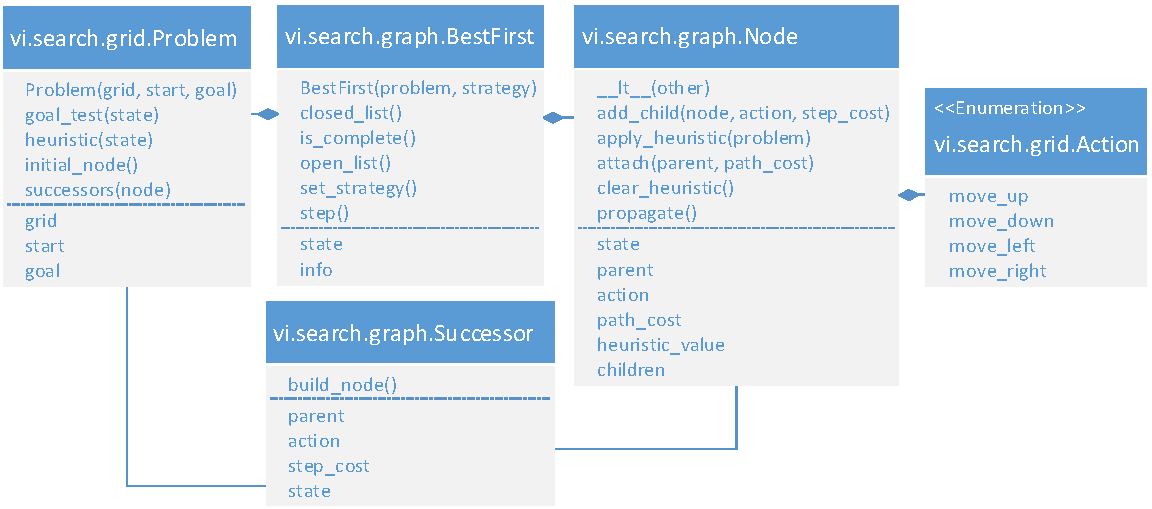
\includegraphics[scale=0.7]{images/vi_class_hierarchy}
\caption{VI Python library classes}
\label{figure:vi_classes}
\end{figure}

\section*{Heuristic function}

The central component of the A* search is the heuristic function which estimates the path cost from a given search space state to the goal state. To guarantee that an A* search finds an optimal solution, the heuristic function must be admissible, meaning that it must never overestimate the path cost to the goal state.

Two popular heuristics for the grid search problem is the Manhattan distance and the Euclidean distance. The Manhattan distance is given by $\textit{abs}(g_x - s_x) + \textit{abs}(g_y - s_y)$ where $g$ is the goal state and $s$ is the given state. Given our grid problem where only vertical and horizontal movement is allowed, the Manhattan distance is not only an admissible heuristic, but also a perfect heuristic since its value will always be the shortest path between a cell in the grid and the goal cell. However since our problem also includes obstacles, the heuristic estimate will not always match the actual path cost as it assumes that all grid cells are traversable.

The Euclidean heuristic uses the straight-line distance between two grid cells as the estimate to the goal. It is given by $\sqrt{(g_x - s_x)^2 + (g_y - s_y)^2}$. It is an admissible heuristic for the problem, but it will underestimate the cost to the goal whenever the starting cell is on a different row or column than the goal.

Table~\ref{table:vi_generated_nodes} shows the Manhattan heuristic outperforming the Euclidean heuristic in all scenarios. If the problem was modified to allow diagonal movements the heuristics would be more equal in their performance.

\begin{table}
\centering
\begin{tabular}{c|ccccc}
Scenario & BFS & DFS & Dijkstra & A* Manhattan & A* Euclidian \\
\hline
0        &  73 &  73 &       73 &           73 &           73 \\
1        & 291 & 296 &      293 &          190 &          256 \\
2        & 344 & 282 &      344 &          215 &          341 \\
3        &  57 &  50 &       56 &           44 &           50 \\
4        &  62 &  58 &       62 &           58 &           59 \\
5        & 273 & 227 &      271 &          233 &          246 \\
\end{tabular}
\caption{Nodes generated for different search strategies}
\label{table:vi_generated_nodes}
\end{table}

\section*{Generating successor states}

``A.I. -- A Modern Approach'' suggests an interface between the search and the problem consisting of the functions \texttt{problem.ACTIONS(node.STATE)}, \texttt{problem.RESULT(parent.STATE, action)} and \texttt{problem.STEP-COST(parent.STATE, action)}. After initially attempting to follow the same abstraction I found it problematic since the work involved in the operations can for many problems be overlapping. For example generating the list of valid actions for a state in the grid problem requires generating the resulting states.

My attempt at a more general interface is a single \texttt{problem.SUCCESSORS} function which does not return a list of successor nodes; but which generates \texttt{Successor} objects representing each valid successor to the given search node. The \texttt{Successor} object contains all information necessary to construct the corresponding \texttt{Node} object, as well as the step cost from the parent node to the successor node.

The \texttt{Successor} abstraction makes it possible to avoid building \texttt{Node} objects when the successor state is not unique. When adding the newly created or existing node object representing the successor state as a child in the parent node; the action and step cost needed to reach the child are also stored. Whenever a child node is later reattached to a parent node the step cost and action information will already be available.

Building the right trade-offs in the interface between what is computationally efficient and memory-efficient will depend on the problem. The focus in this abstraction has been on semantic correctness and avoiding redundant computation.

\end{document}

